En este apartado se analizarán los tiempos de ejecución, el consumo de memoria y la calidad de las soluciones obtenidas por cada algoritmo, considerando los distintos tipos y tamaños de grillas. Además, se compararán los puntajes obtenidos por Greedy y Programación Dinámica, junto con sus tasas de éxito y fallos al encontrar caminos válidos. Los valores de memoria representan el consumo máximo del proceso durante su ejecución, incluyendo el almacenamiento de las grillas.

Antes de entrar en la parte de análisis, es importante mencionar como funciona cada algoritmo implementado ya que cada uno encuentra el mejor camino (o puede ocurrir que no como en el caso de Greedy) de forma diferente. Greedy toma decisiones locales, seleccionando en cada movimiento la casilla que entrega el mayor beneficio inmediato, sin considerar las consecuencias futuras. En el caso de Fuerza Bruta, genera todas las secuencias posibles de movimientos y evalúa los caminos válidos para encontrar el que entrega el mayor puntaje. Para finalizar, Programación Dinámica considera las distintas posibilidades de caminos mediante el cálculo y almacenamiento de los mejores puntajes para cada posición y cantidad de vidas disponibles, permitiendo encontrar el camino óptimo sin tener que evaluar todos los caminos posibles como lo hace Fuerza Bruta.

\subsection{Tiempos de ejecución}

Ahora se analizarán los tiempos de ejecución de cada algoritmo en todos los casos de prueba (libre, murallas, minas y mixta). A continuación se muestran los gráficos de los resultados obtenidos.

\begin{figure}[H]
    \centering

    \begin{minipage}{0.48\textwidth}
        \centering
        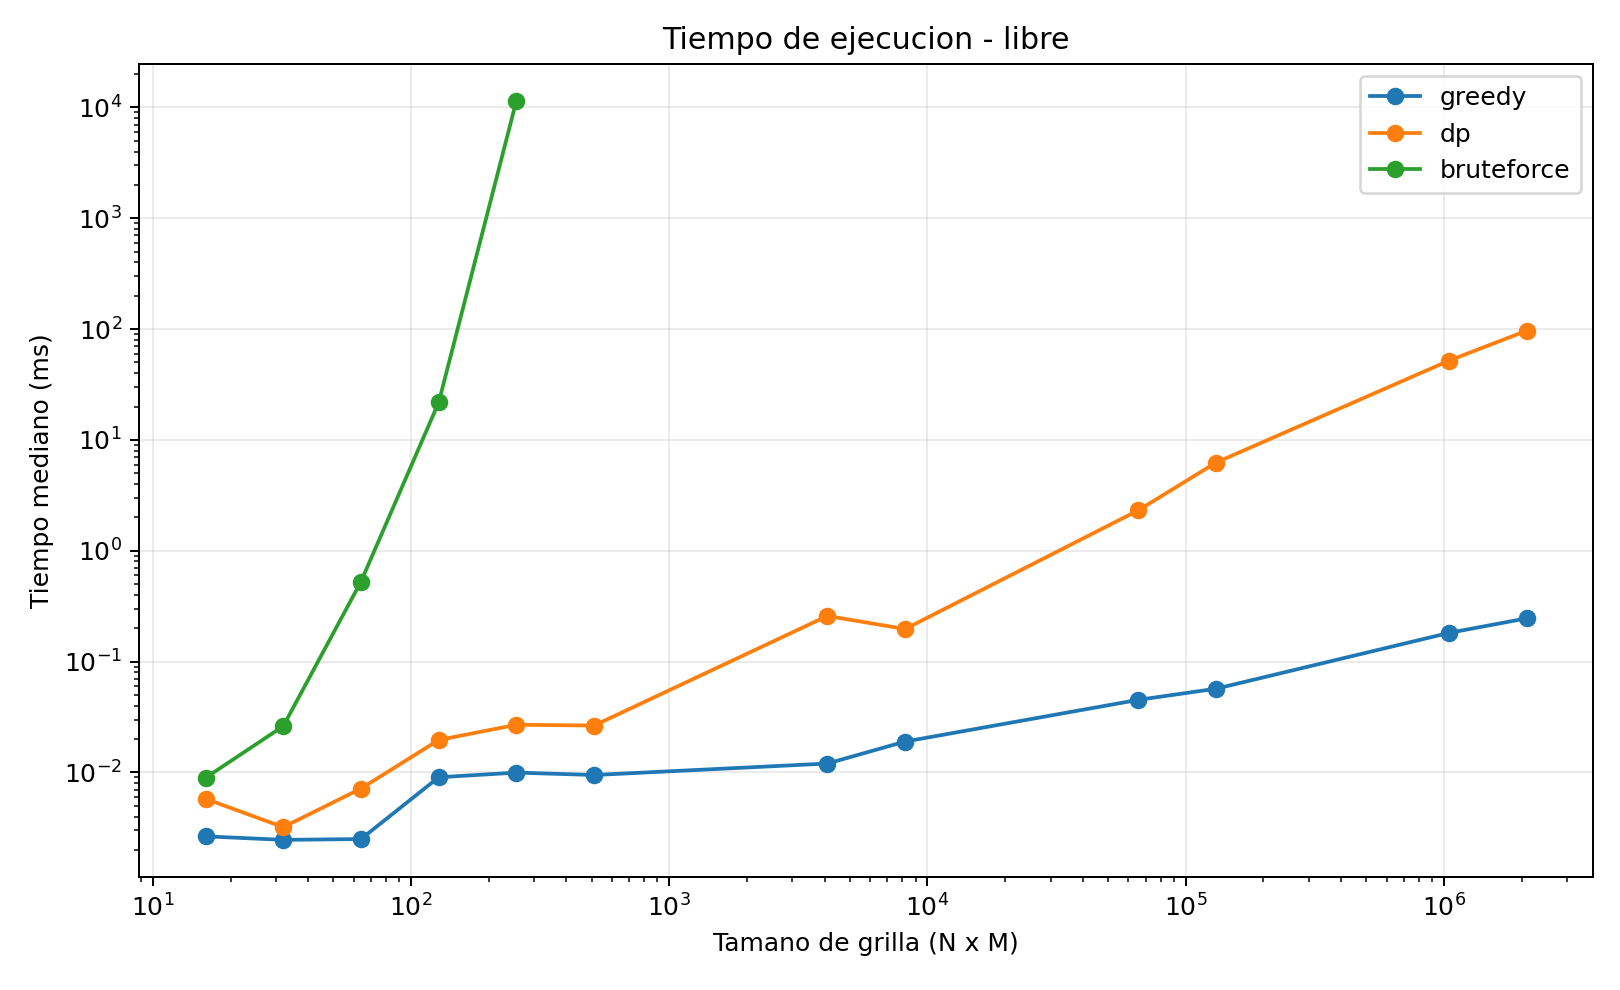
\includegraphics[width=0.90\linewidth]
        {plots/tiempo_libre.png}
        \small (a) Grillas libres
    \end{minipage}
    \hfill
    \begin{minipage}{0.48\textwidth}
        \centering
        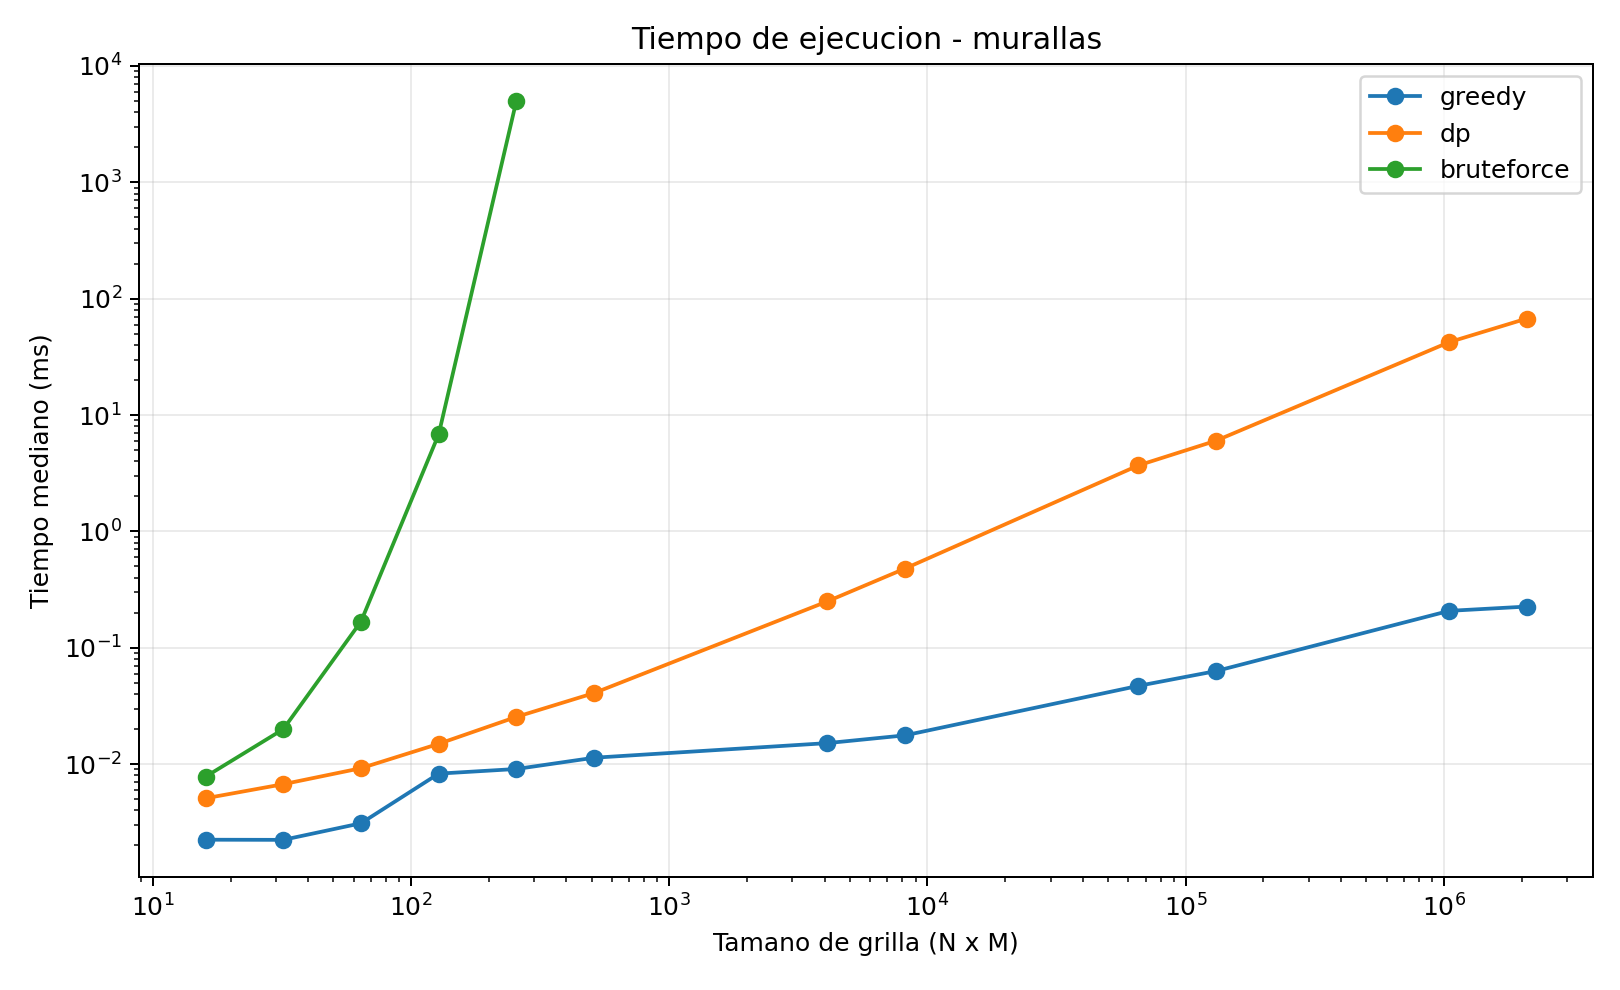
\includegraphics[width=0.90\linewidth]
        {plots/tiempo_murallas.png}
        \small (b) Grillas con murallas
    \end{minipage}

    \caption{Tiempos de ejecución en grillas libres
    y con murallas.}
    \label{fig:tiempos1}
\end{figure}

\begin{figure}[H]
    \centering

    \begin{minipage}{0.48\textwidth}
        \centering
        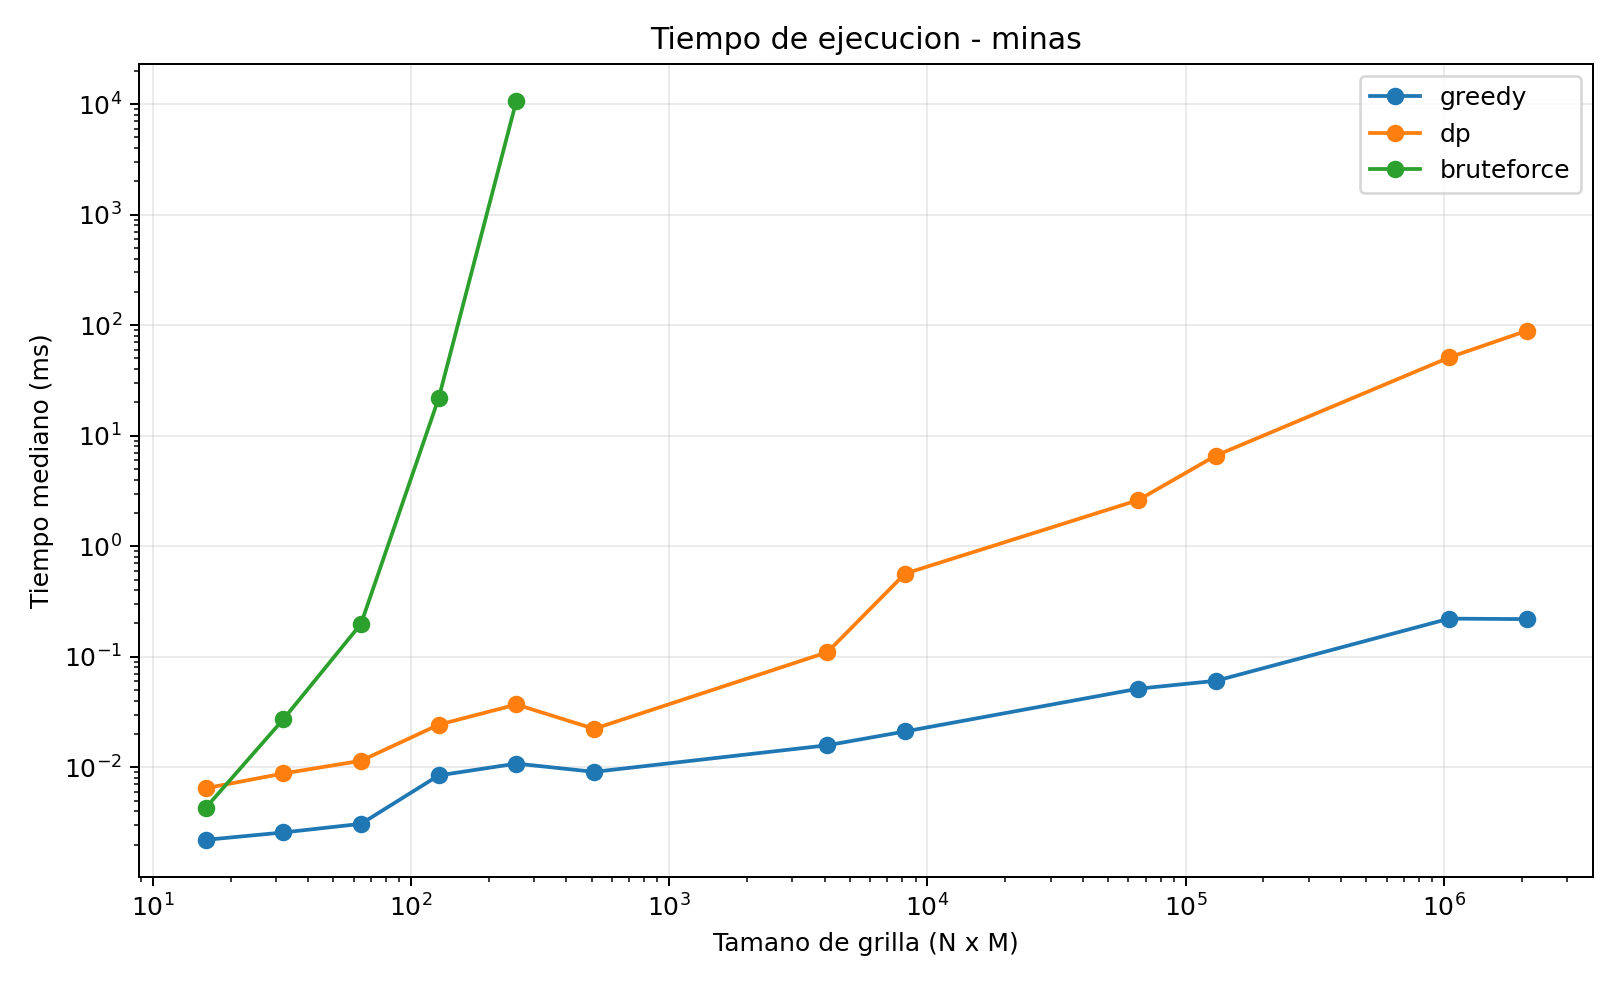
\includegraphics[width=0.90\linewidth]
        {plots/tiempo_minas.png}
        \small (a) Grillas con minas
    \end{minipage}
    \hfill
    \begin{minipage}{0.48\textwidth}
        \centering
        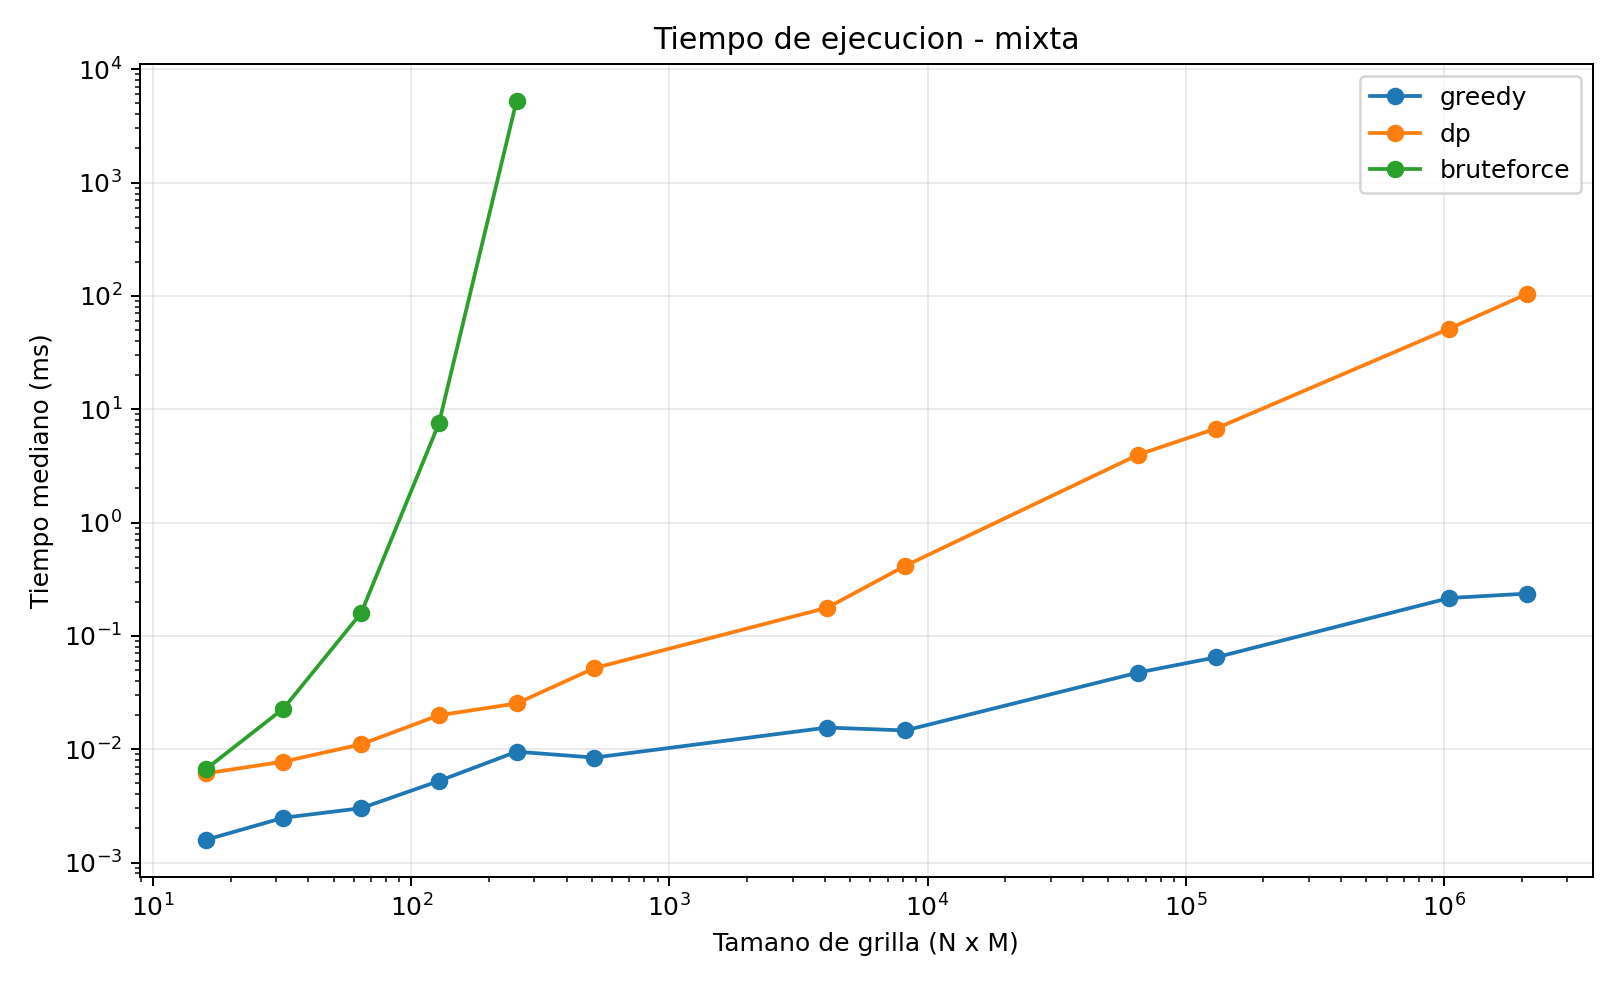
\includegraphics[width=0.90\linewidth]
        {plots/tiempo_mixta.png}
        \small (b) Grillas mixtas
    \end{minipage}

    \caption{Tiempos de ejecución en grillas
    con minas y mixtas.}
    \label{fig:tiempos2}
\end{figure}

Tanto en los gráficos a y b de las figuras 1 y 2, se puede ver que Greedy tiene menores tiempos de ejecución en los distintos tipos de grillas, lo que concuerda con su complejidad teórica de O(N+M), esto ya que toma decisiones locales sin tener que evaluar todas las posibilidades lo que hace que solo necesite realizar N+M-2 movimientos para llegar al destino. En el caso de Programación Dinámica, este algoritmo presenta tiempos mayores que Greedy, pero mantiene un crecimiento moderado a medida que aumenta el tamaño de las grillas, lo que concuerda con su complejidad O(NMV), ya que calcula y almacena los mejores resultados obtenidos para cada estado y evita repetir cálculos.

En comparación, Fuerza Bruta presenta un aumento notorio en sus tiempos de ejecución a medida que crece el tamaño de las grillas, lo que se relaciona con su complejidad teórica de \(O\left((N+M)\binom{N+M-2}{N-1}\right)\). Esto ya que este último algoritmo, genera todas las secuencias posibles de movimientos y evalúa cuáles corresponden a caminos válidos, por lo que la cantidad de posibilidades aumenta rápidamente. En las grillas de 16×16, sus tiempos llegan a superar los 10 segundos, mientras que los otros algoritmos registran tiempos inferiores a 0,1 ms para ese mismo tamaño.

Finalizando este apartado de los tiempos de ejecución, se observa que en las grillas más grandes de 1024×2048, Greedy registra aproximadamente 0,25 ms y Programación Dinámica alrededor de 95 ms, mientras que Fuerza Bruta no fue ejecutada debido a la restricción de \(N+M \leq 32\) establecida en la tarea.

\subsection{Consumo de memoria}

En este punto, se estudiará el consumo máximo de memoria
registrado durante la ejecución de los tres algoritmos,
tomando en cuenta los distintos tamaños de grillas.

\begin{figure}[H]
    \centering
    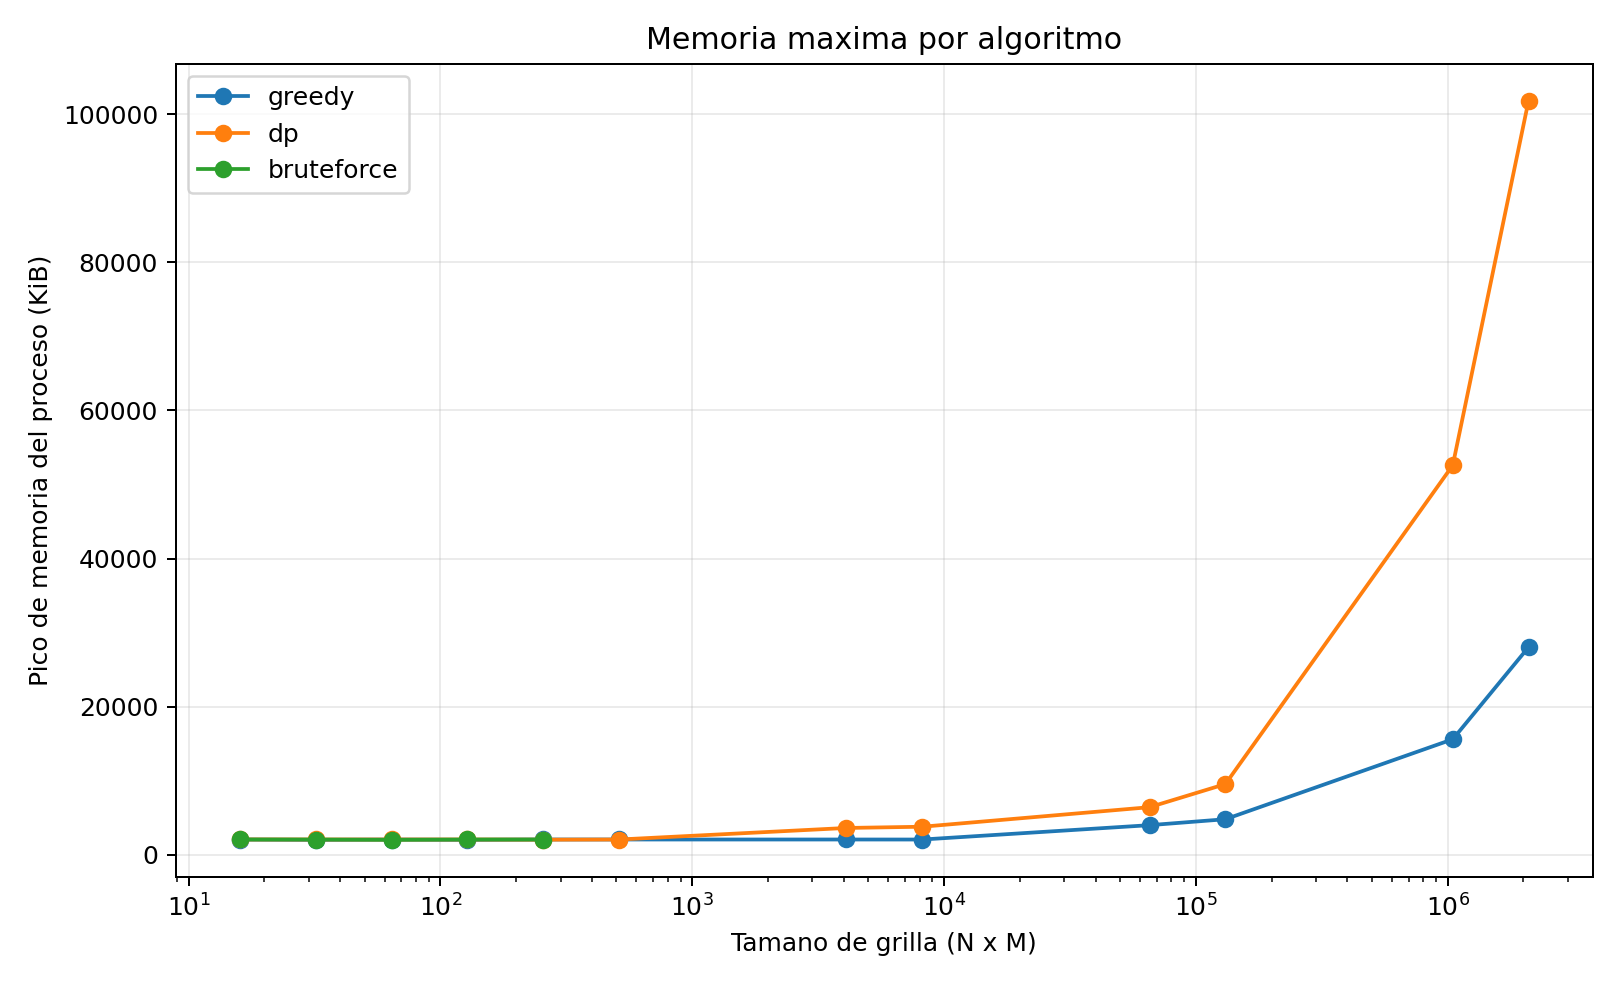
\includegraphics[width=0.60\textwidth]{plots/memoria_algoritmos.png}
    \caption{Consumo máximo de memoria según el tamaño de las grillas.}
    \label{fig:memoria}
\end{figure}

En la Figura 3 se puede ver que Programación Dinámica tiene el mayor consumo de memoria a medida que aumenta el tamaño de las grillas, lo que se relaciona con su complejidad espacial de O(NMV), debido a que necesita almacenar los mejores puntajes y la información necesaria para reconstruir los caminos seleccionando los estados óptimos de las posiciones escogidas. Por otro lado, Greedy y Fuerza Bruta tienen una complejidad espacial auxiliar de O(N+M), ya que almacenan principalmente los caminos y las variables necesarias durante su ejecución.

En las grillas de 1024×2048, Programación Dinámica alcanza aproximadamente 102.000 KiB, mientras que Greedy registra alrededor de 28.000 KiB.

Es importante mencionar que los valores obtenidos representan el consumo máximo de memoria de cada algoritmo en cada grilla, incluyendo el almacenamiento de estas, por lo que no corresponden únicamente a la memoria auxiliar utilizada por cada algoritmo.

\subsection{Calidad de las soluciones}

En este punto, se revisará la diferencia entre los puntajes obtenidos por Greedy y Programación Dinámica, considerando los dominios D10 y D1000. Con el objetivo de analizar qué tan cerca está Greedy de encontrar el camino óptimo, comparando su puntaje con el obtenido por Programación Dinámica.

\begin{figure}[H]
    \centering

    \begin{minipage}{0.48\textwidth}
        \centering
        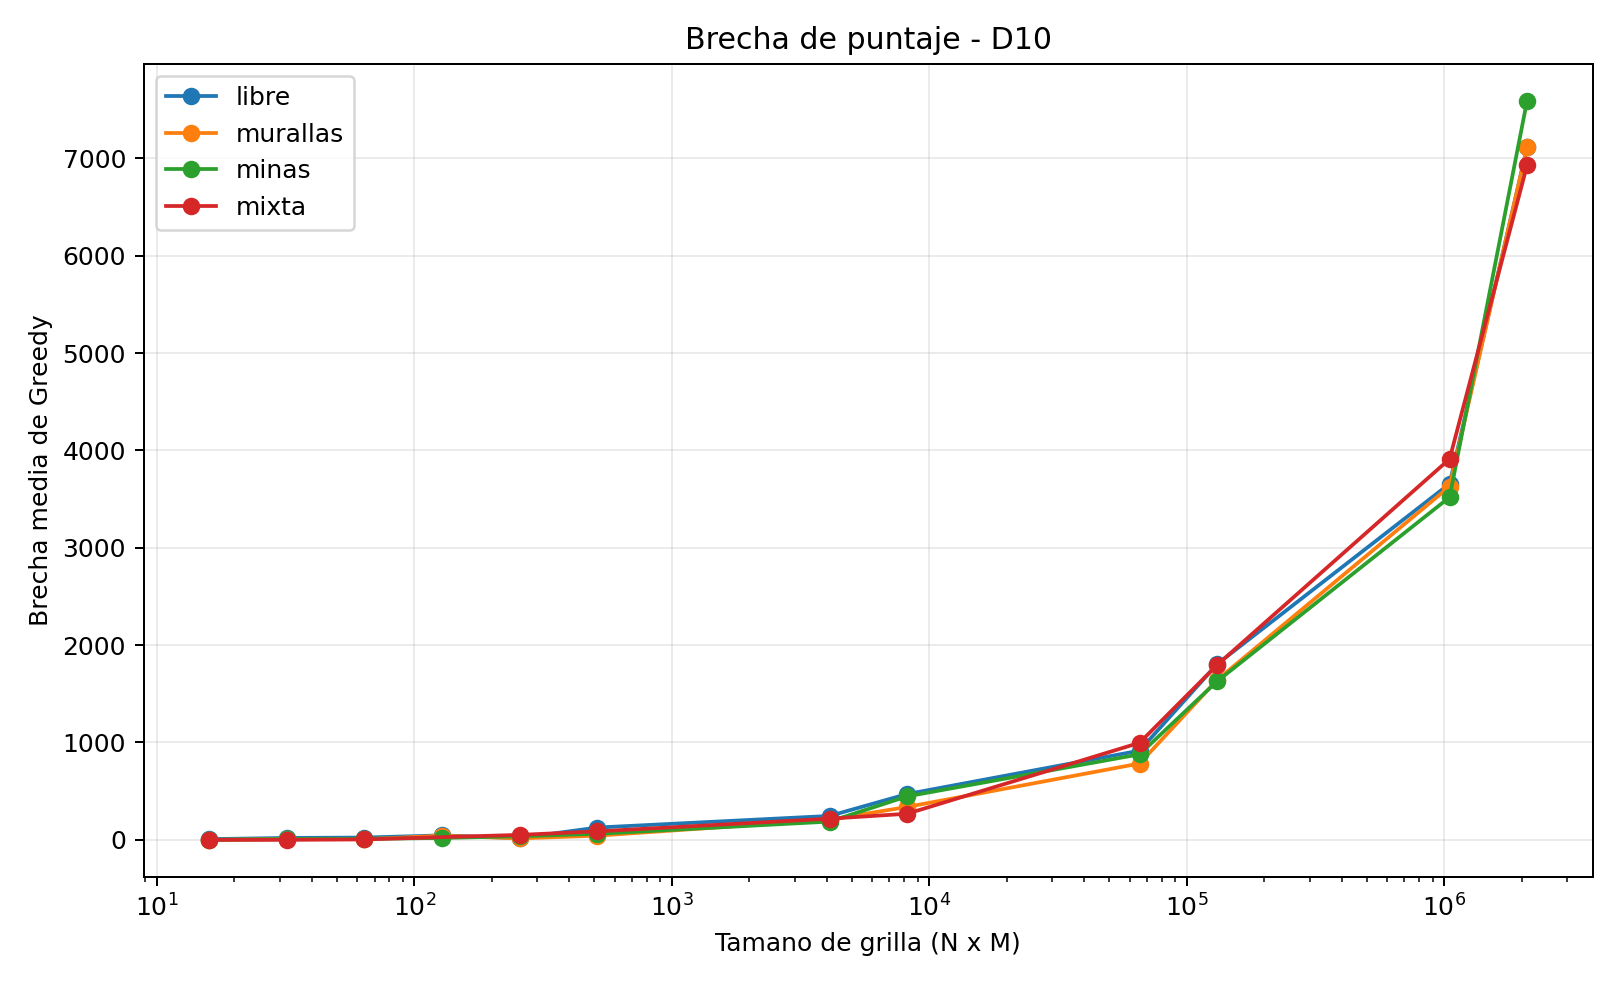
\includegraphics[width=0.95\linewidth]{plots/brecha_D10.png}
        \small (a) Dominio D10
    \end{minipage}
    \hfill
    \begin{minipage}{0.48\textwidth}
        \centering
        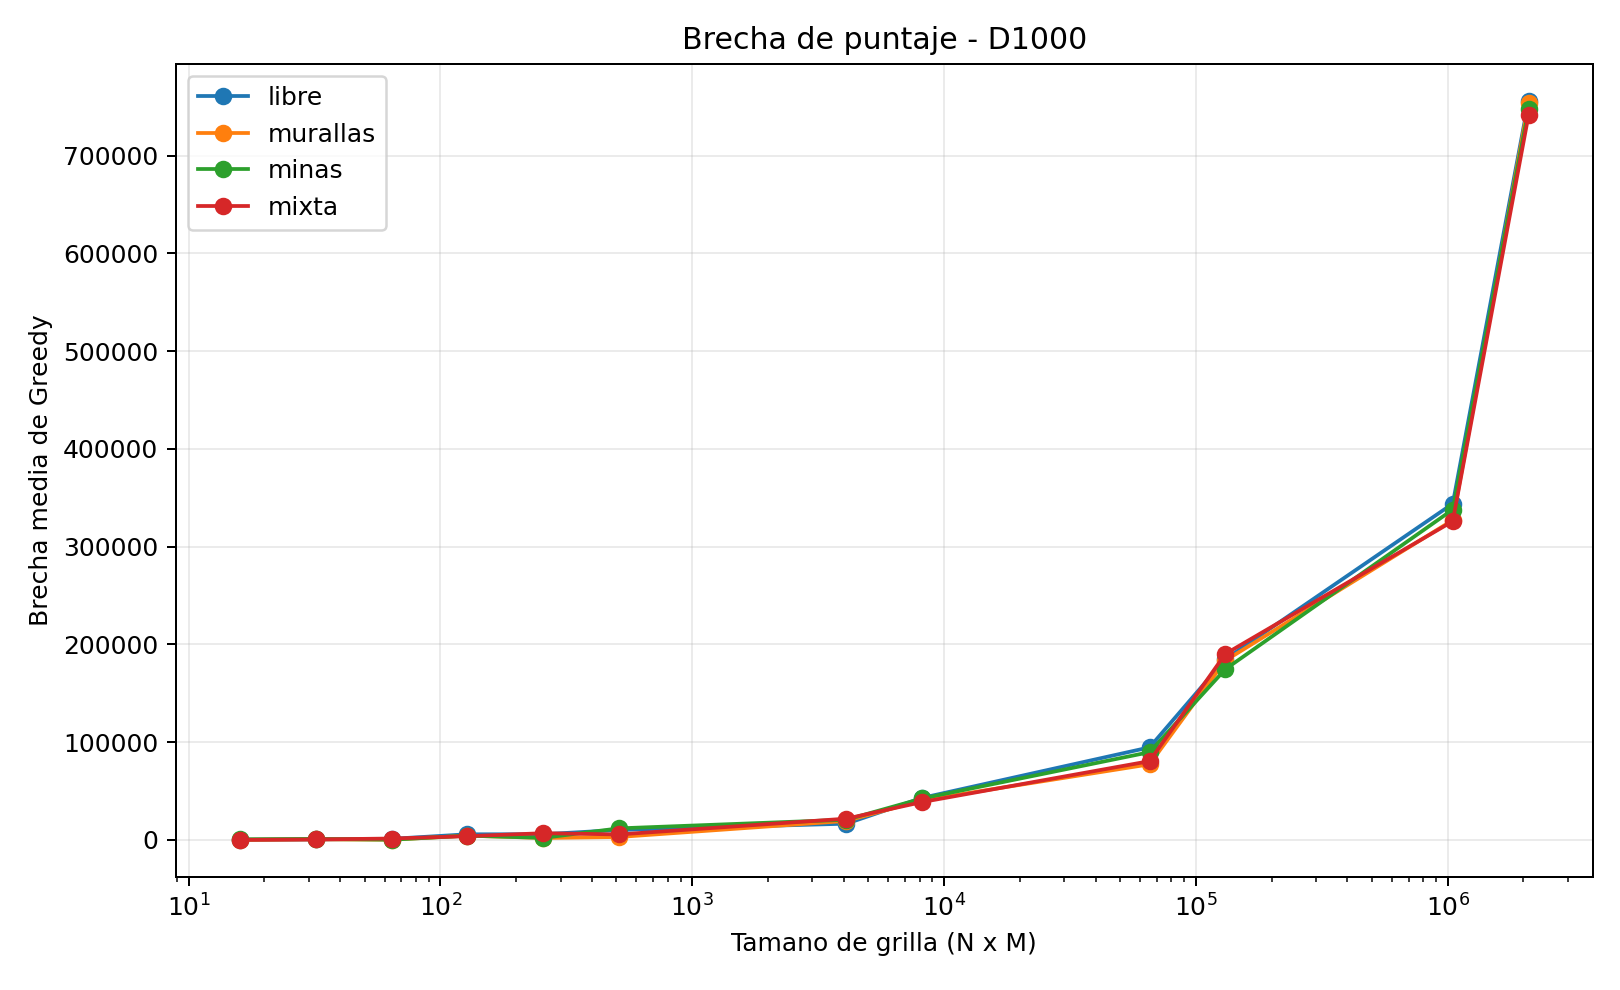
\includegraphics[width=0.95\linewidth]{plots/brecha_D1000.png}
        \small (b) Dominio D1000
    \end{minipage}

    \caption{Brecha media de puntaje entre Greedy
    y Programación Dinámica.}
    \label{fig:brechas}
\end{figure}

En la Figura 4 se puede ver que la diferencia entre los puntajes obtenidos por Greedy y Programación Dinámica aumenta de forma considerable a medida que crece el tamaño de las grillas. Esto porque Greedy toma decisiones locales sin considerar los beneficios futuros, mientras que Programación Dinámica evalúa los distintos estados para encontrar el camino con el mayor puntaje posible.

En las grillas de 1024×2048, la diferencia de puntaje media del dominio D10 alcanza valores entre 6.900 y 7.600 puntos, mientras que en D1000 se encuentran alrededor de 740.000 a 760.000 puntos. Esta diferencia entre los dominios ocurre ya que D1000 utiliza valores de mayor magnitud, lo que genera diferencias absolutas de puntaje más altas.

Estos resultados demuestran que, aunque Greedy presenta menores tiempos de ejecución, esto no significa que encuentre las mejores soluciones, ya que sus decisiones locales pueden llevarlo a obtener puntajes peores al óptimo. Pero en comparación a Programación Dinámica, este último requiere un mayor tiempo de ejecución, pero garantiza encontrar el camino con el mayor puntaje posible.

Es importante mencionar que estas diferencias se calcularon únicamente en las instancias donde Greedy logró encontrar una solución válida.

\subsection{Tasa de éxito y fallos}

Como último punto, se analizará la capacidad de Greedy y Programación Dinámica para encontrar caminos válidos en los distintos tipos de grillas, con el objetivo de determinar con qué frecuencia logran llegar al destino. Además, se utilizarán los resultados de Programación Dinámica para comprobar que los fallos de Greedy ocurren incluso cuando existe una solución válida.

\begin{figure}[H]
    \centering

    \begin{minipage}{0.48\textwidth}
        \centering
        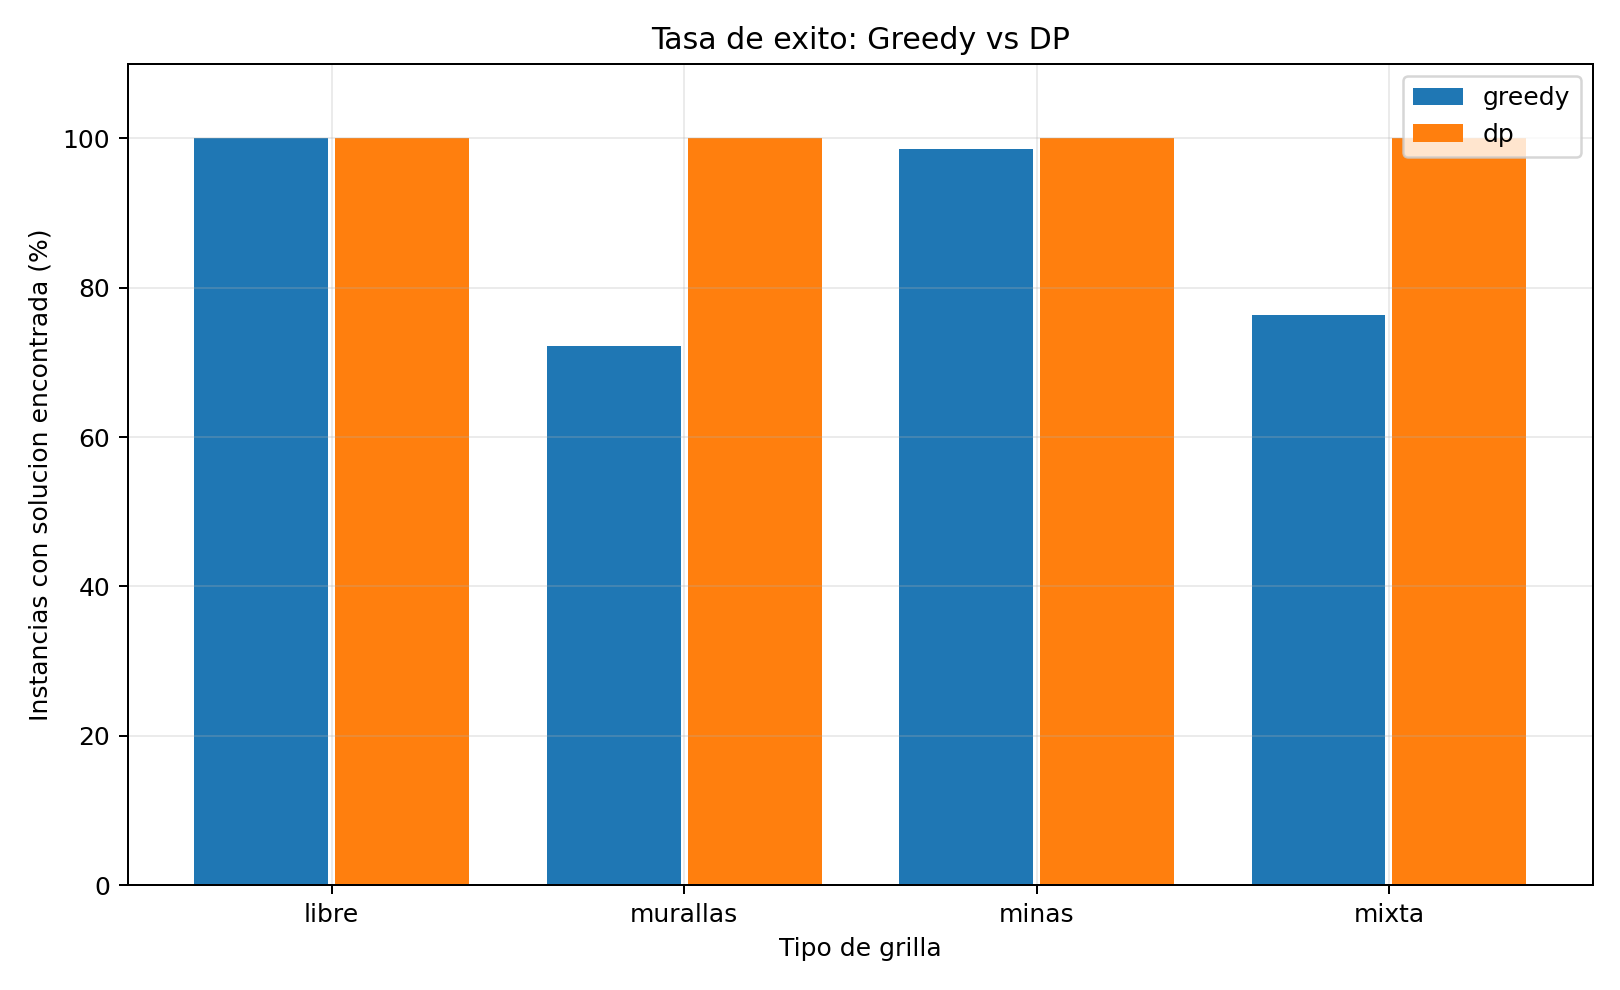
\includegraphics[width=0.95\linewidth]{plots/exito_greedy_dp.png}
        \small (a) Tasa de éxito
    \end{minipage}
    \hfill
    \begin{minipage}{0.48\textwidth}
        \centering
        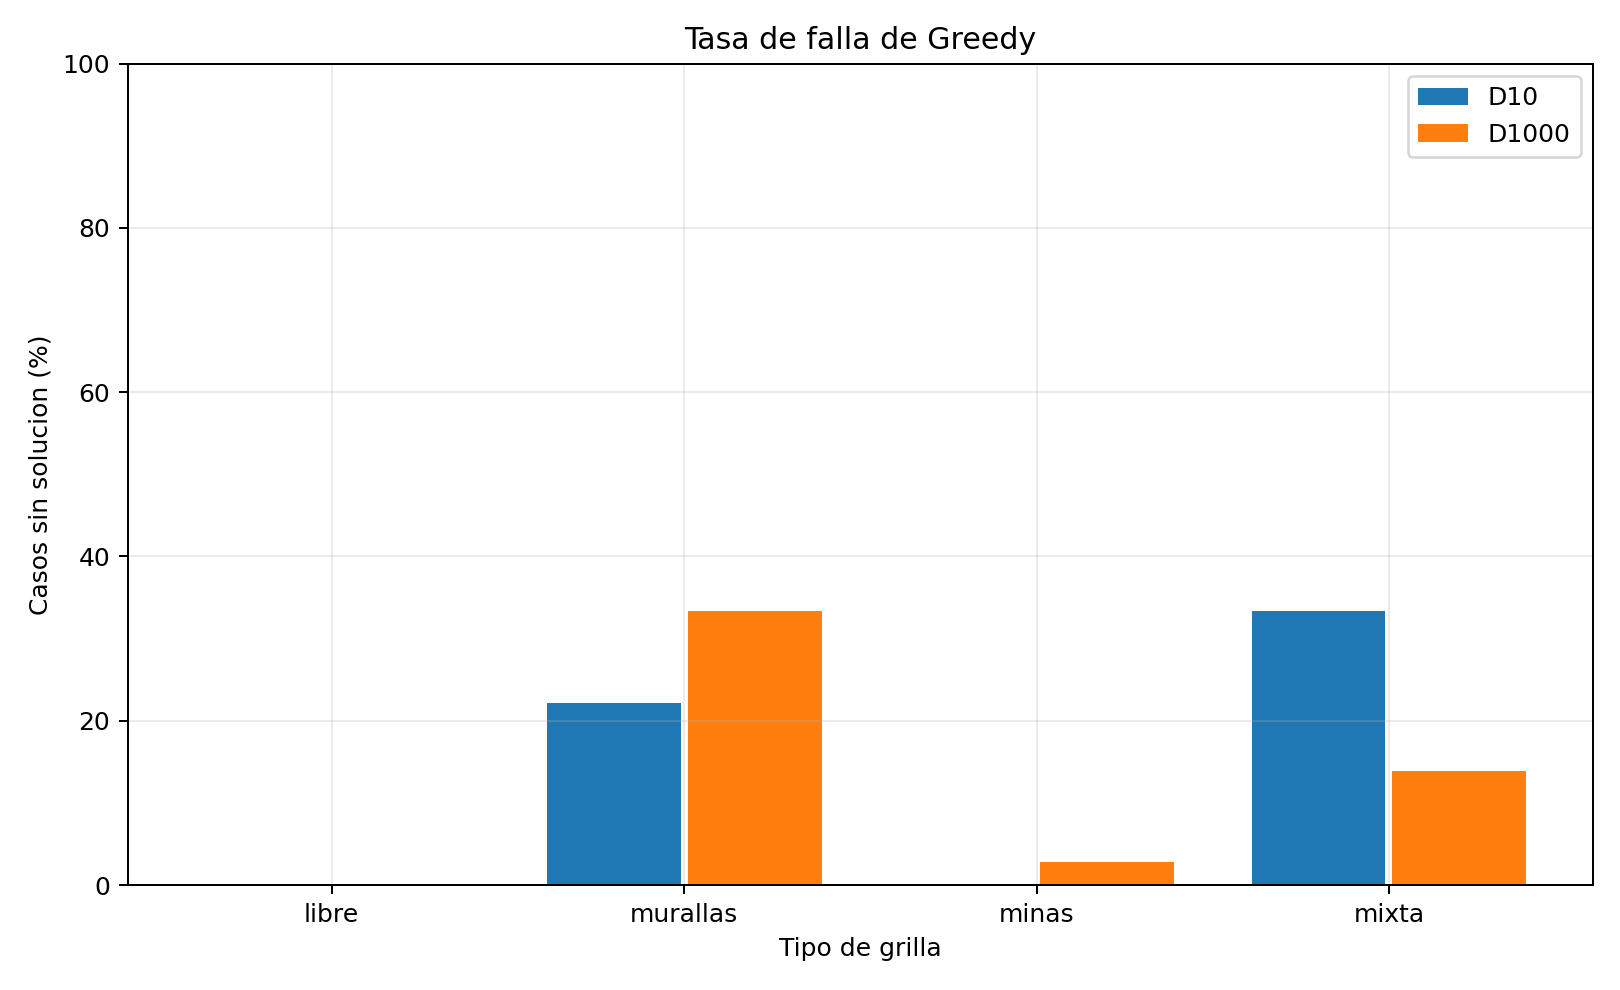
\includegraphics[width=0.95\linewidth]{plots/fallas_greedy.png}
        \small (b) Tasa de fallos de Greedy
    \end{minipage}

    \caption{Tasas de éxito y fallos en la búsqueda de caminos válidos.}
    \label{fig:exito_fallos}
\end{figure}

En la Figura 5 se observa que Programación Dinámica encontró una solución en las 288 instancias evaluadas, alcanzando un 100\% de éxito. En cambio, Greedy presentó fallos principalmente en las grillas con murallas y mixtas, donde obtuvo aproximadamente un 72\% y 76\% de éxito, respectivamente. Esto ocurre porque sus decisiones locales pueden llevarlo a caminos sin salida, incluso cuando existe una solución válida. En cambio, Programación Dinámica considera las distintas posibilidades para encontrar un camino válido y de mayor puntaje, siempre que exista una solución.

Finalmente, se realizó una comparación entre los resultados de Fuerza Bruta y Programación Dinámica en las 120 instancias donde ambos algoritmos fueron ejecutados. En todos los casos se obtuvo el mismo puntaje y resultado de factibilidad, sin encontrar diferencias, lo que respalda experimentalmente la correcta implementación de ambos algoritmos.